%Part of/Parte di https://github.com/f-dinucci/appuntiMeccanicaFluidi/
%License/Licenza Creative Commons Attribution-ShareAlike 4.0 International (CC BY-SA 4.0) - attribution/attribuzione Francesco Di Nucci
%See also/Vedere anche https://creativecommons.org/licenses/by-sa/4.0/ and/e https://creativecommons.org/licenses/by-sa/4.0/legalcode
%
\section{Introduzione ai sistemi continui}
%
\subsection{Meccanica Classica e Meccanica dei Continui}
Nella meccanica classica\footnote{cioè non quantistica e non relativistica} ci si riferisce ad un sistema discreto: corpi che esercitano forze di varia natura l'uno sull'altro e subiscono delle accelerazioni per via di queste forze.
Nella meccanica dei fluidi si utilizza invece il concetto di sistema continuo (sistema in cui le proprietà variano con continuità nello spazio).
Questo vuol dire che nei fluidi le proprietà dipendono dal tempo e dalle coordinate spaziali, cioè sono $f(x, y, z, t)$, mentre nella meccanica classica dipendono solamente dal tempo, sono cioè $f(t)$.
%
	\begin{equation*}
		\begin{aligned}
			&\text{Sistema discreto} \quad  f(t)  \\ %& per allineamento
			&\text{Sistema continuo} \quad f(x, y, z, t)
		\end{aligned}
	\end{equation*}
%
Per affrontare i problemi relativi ai fluidi si vuole arrivare a scrivere delle equazioni differenziali, che  per il motivo di cui sopra saranno equazioni differenziali ordinarie \textit{in più variabili}.
%
\subsection{Volume di controllo}
Nello studio dei solidi si ha una configurazione di riferimento che può cambiare per via di una deformazione, i fluidi\footnote{che includono tutto ciò che non è solido, quindi liquidi, gas, vapori ecc.} invece non hanno forma: scorrono con l'applicazione di una forza anche minima.
Si introduce quindi il concetto di \textit{volume di controllo}: si ``fissa lo sguardo'' su di un volume in particolare, nel quale si vuole stabilire un bilancio\footnote{in parole povere capire cosa entra e cosa esce, valutare le grandezze in ingresso ed in uscita}.
	\begin{figure}[H]
		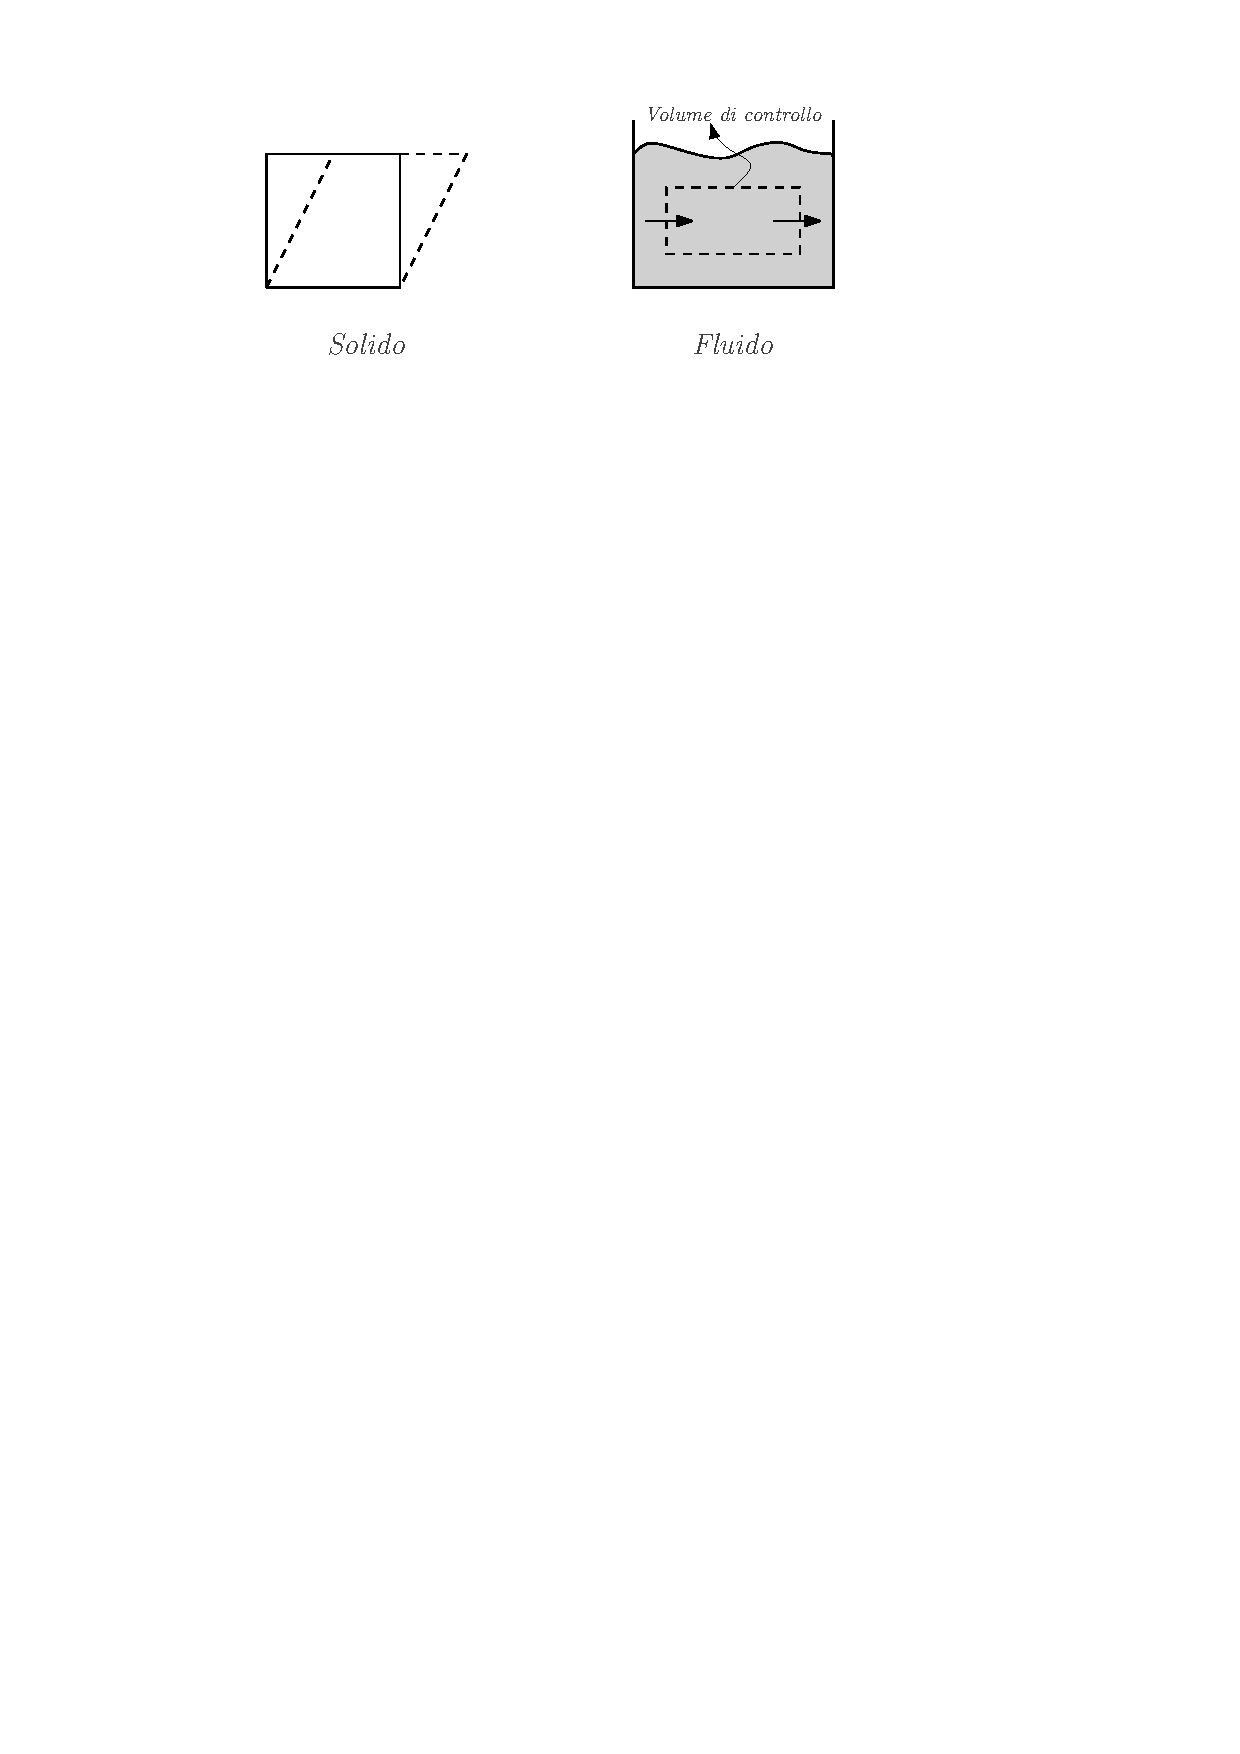
\includegraphics[scale=0.9]{./1.1 Introduzione ai sistemi continui/1.1-1}
		\centering
		\caption{Confronto tra solido e fluido}
	\end{figure}
Mentre nei solidi le proprietà sono riferite alle particelle, nei fluidi queste ultime entrano ed escono continuamente dal volume di controllo\footnote{che non è un volume di fluido}, quindi le coordinate spaziali e le proprietà in generale si riferiscono al volume di controllo (e non alle particelle), sul quale si stabiliranno dei bilanci.
Da notare che le due descrizioni non sono mutuamente esclusive, matematicamente si possono descrivere i solidi utilizzando dei volumi di controllo e dei fluidi riferendosi a delle particelle che in un dato momento si trovavano in una certa posizione. 
Da un punto di vista formale la descrizione solitamente utilizzata per i solidi è detta \textit{lagrangiana}, quella per i fluidi \textit{euleriana}.
%
\subsection*{Bibliografia 1.1}
\cite[Cap.\ 1.1, 4.1]{CengelCimbala}\\
\cite[Cap.\ 1.1]{LuchiniQuadrio}\\
\cite[Cap.\ 1.1]{PnueliGutfinger}